\documentclass{article}
\usepackage{graphicx}
\usepackage[margin=1in]{geometry}
\usepackage{subcaption}

\begin{document}

\title{Simulation Write Up{}}
\author{Amy Solman}

\maketitle

\section{Aims}
To test the hypothesis that the predictions made by Chisholm’s model are statistically significantly similar to the results of my island simulation. 

To test the hypothesis that, as island area increases, it transitions from a niche-structured regime, to a colonisation-extinction balance regime. 

\section{Methods}

\subsection{Simulation Design}

I developed a simulation which took the inputs of meta community size (J\_meta), speciation rate (nu), the number of different migration rates to be simulated (num\_m\_rates), the maximum niche size (max\_k\_size), the maximum number of niches to be simulated (max\_k\_num), the amount of time the simulation is to be run for (wall\_time) and the name of the files in which to store the simulation data (output\_file\_name).\bigskip

For each simulation I began by generating a metacommunity, using the function coalescence\_test written by James Rosindell. The function took the inputs of J\_meta and nu, and output a vector of simulated species abundances. I passed the abundance vector to a second function (metacommunity), that repeated a unique species number by each number of the abundance vector (for example abundance vector (5,4,1,1) gives community (1,1,1,1,1,2,2,2,2,3,4)). \bigskip

The size of each simulation island was determined by the number of niches multiplied by the size of each niche. Each niche on each island was generated through the niche\_info function. The function took the inputs of migration rate (m), speciation rate (nu) and niche size (k\_size). Each niche started off with a completely homogenous community of species 1 by k\_size (for example k\_size = 5, niche community = 1,1,1,1,1). The starting community of each niche, as well as speciation and migration rate were stored in an output list. The niche\_info function run through the niches function, and repeated from 1 to maximum niche size (max\_k\_num), outputting island communities that grew in size from one niche to max\_k\_num (for example, max\_k\_num = 3 would produce 3 islands consisting of 1 niche, 2 niches and 3 niches, each of k\_size). \bigskip

The niches function was repeated through the multi\_islands function, from 1 to the number of different migration rates (num\_m\_rates). Migration rates started at 0.002 and increased by 0.002 each time. The multi\_islands function also generated a unique species list (unique\_sp) that calculated the number of unique species across all niches of each islands and stored this data, along with each island community, speciation and migration rate. The output of multi\_islands was a list of islands, along with the communities of each of their niches, the speciation and migration rates of each niche, and the total number of unique species on that island. \bigskip
 
 \begin{figure}[h!]
\centering
  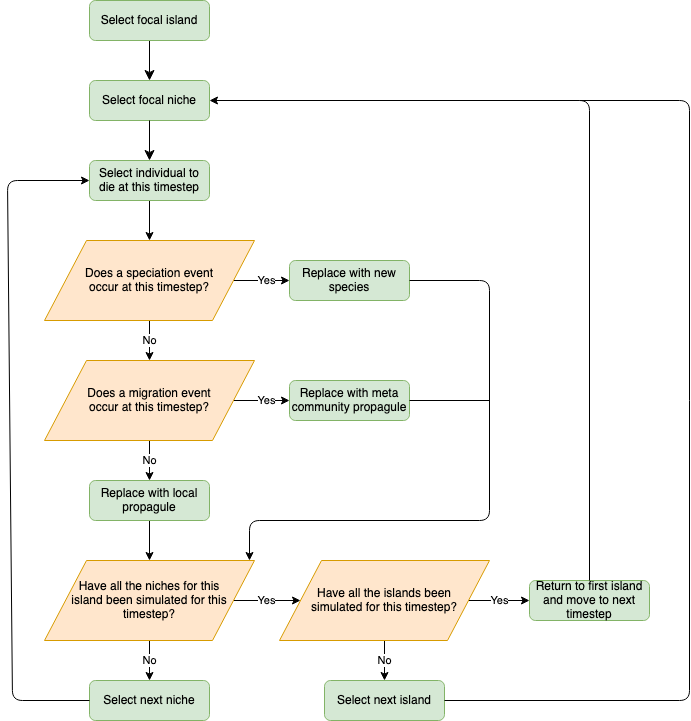
\includegraphics[scale=0.4]{../../Other/neutral_flowchart.png}
  \caption{Flowchart of simulation design}
  \label{fig:Flowchart}
\end{figure}
 
I then started a timer. While the timer was less than the wall\_time the cluster\_run\_function would continue to loop through the communities. At each time step, each island is chosen and each niche is passed through the simulation\_one\_timestep function.  An individual within that niche chosen to die and with probability speciation (0.001) a new species is generated to take its place. With probability migration rate, an individual chosen from the metacommunity replaces the dead individual. With probability 1 – speciation rate + migration rate, an individual is chosen from within the niche to replace the dead individual. Once all niches for one island have had simulation\_one\_timestep act upon it, the simulation moves to the next island. Once all niches on all islands have passed through simulation\_one\_timestep, the simulation moves to the next timestep. Every 10000 timesteps the species richness of each island is recorded and stored. The simulation continues until wall\_time is reached. Each run of the cluster\_run\_function output the final communities of each island and a timeseries of species richness, along with the number of timesteps the simulation had progressed through, the total time spent on the simulation, the size of the metacommunity, the speciation rate and the output file name). \bigskip

A second R script (ClusterCode.R) was written to source the ClusterSim.R functions. The cluster job index number was applied to the value iter. The value iter was given to i and i was used to set a seed for the simulation. Output\_file\_name was given the value of simulation\_timeseries\_i, to give a different output filename for each iteration of the simulation. The cluster\_run\_function was then called (see Table 1 for input parameters). \bigskip

Finally, a bash script (ClusterRun.sh) was used to set the wall\_time for the simulation in the cluster (24:00:00). This script called the ClusterCode.R script to run on the cluster, and output the 100 simulation output files to \$HOME directory. \bigskip

I ran my simulation on the Imperial College London high-performance computing cluster for 23 hours. The simulation was repeated 100 times. Each simulation generated 3375 islands (num\_m\_rates x max\_k\_size x max\_k\_num). 

\subsection{Data Preparation and Timeseries Plots}
After downloading my simulation results from the cluster, I imported each file into DataPrep.R script. I isolated the data from each island and create a data frame with simulation number, migration rate, area, number of niches and number of species. I created a second data frame with simulation number, island number, migration rate, timestep and species richness timeseries for each island. I then saved the final island data and timeseries data to separate csv files. \bigskip

To ensure the simulation had run long enough for each island to reach dynamic equilibrium I wrote a timeseries plotting script (TimeseriesPlot.R). I loaded the R packages GGPlot2 and gridExtra to create my timeseries plots and put save multiple plots to one pdf file respectively. I imported the timeseries data from my simulations (SimTimeseriesPlotData.csv). I then isolated the data from simulations 25, 50 and 75. I plotted the timeseries data of each island for each simulation, on a three-panel plot.  

\section{Analysis}
For my analysis script (Analysis.R), I loaded the R package broom, to use the tidy() function for accessing the summary statistics of linear models. I imported my final island data (SimModelFitData.csv) and for each island across all my simulations (337,500) I generated an estimated species richness by giving the island area, number of niches, m0 and an estimated theta to the chisholm\_function. The results of my simulation and those estimated by the chisholm\_function was then bound together in a data frame. I also found the mean species richness results for each combination of island area, migration rate and number of niches across all 100 simulations.
  
\subsection{Within Simulation Analysis}

\subsubsection{Repeatability}
I checked the repeatability of my simulation by running a linear model of species richness, with simulation number as independent variable. I then run an ANOVA (analysis of variance) on the linear model of species richness with simulation as the explanatory variance. From this I was able to calculate the repeatability statistic. This is calculated by dividing the among-group variance by the within-group variance, minus the among-group variance. We are calculating the percentage of the total variance that is explained by among-simulation differences. Essentially, we want to make sure there is more within simulation variance than among simulation variance. We want to make sure our simulations are relatively consistent. As the same statistical parameters are being applied to each (speciation rate = 0.001, migration rates 0.003 - 0.045, niche numbers 1-15, niche sizes 1-15) we would expect variation among simulations to be less than variation within simulations. We would expect our simulations to give us consistent results. This allowed me to ascertain to what extent the variability in species richness is explained by differences in the simulations.

\subsubsection{Normaility}
I checked the normality of my simulation data by creating histograms of species richness results. It was necessary to check the normality of my data as I use linear regression in my analysis and it assumes the data are normally distributed. 

\subsubsection{Collinearity}
I assessed the collinearity of my simulation dataset by using the R base function pairs() to produce a scatterplot of matrices. This allowed for visual inspection of the relationships between number of species, migration rate, island area and number of niches. It is important to assess the collinearity of covariates because it can inflate variation. Large amounts of collinearity cause covariates to have larger standard errors and it becomes less likely to detect a significant result. The Variance Inflation Factor (VIF) was calculated to assess if the collinearity between number of niches and island area was within acceptable limits for this analysis. 

\subsubsection{Linear Regression}
Next, I began to assess whether there was a statistically significant relationship between my dependent variable (species richness) and independent variables (area and niches). Firstly, I calculated the mean species richness for each unique set of parameters across all 100 simulations. Then, I z-transformed my area and niche variables so that they could better meet the assumptions of a linear model. Moreover, the intercept statistic for z-standardized data gives us the mean of the dependent sample. I ran a linear model on the mean species data and z-transformed area and niche variables separately, to assess to what extent each explained variation in the dependent variable. I also generated histograms of the residuals of each linear model to check for homogeneity of the variances to validate the assumptions of the regression analyses. I then validated the models by checking the distribution of the residuals. 

\subsubsection{Multivariate Analysis}
I performed a multivariate analysis of the mean simulation data, including number of niches, island area and migration rate. This allowed me to assess to what extent the three independent variables were important for predicting species richness. I performed a second multivariate analysis, including niche number and island area only. I plotted the results of both of these models to check the distribution of the residuals.

\subsection{Simulation/Model Analysis}

\subsubsection{Outliers}
For my analysis, I began by checking the data for outliers. I did this by creating boxplots of species richness’s generated by my simulation and those generated by the chisholm\_function. By ensuring the number of possible outliers is low in comparison to sample size, I ensured the data would not be skewed by anomalous results.

\subsubsection{Range, variance, standard deviation and standard error}
I found the range, variance, standard deviation and standard error of both my simulation and the chisholm\_function. Homogeneity of variances is an important assumption for certain statistical tests such as ANOVA and regression analysis. In my analysis I will be working mostly with regression analysis, wherein it is more important to look at the variances of the residuals. 

\subsubsection{Paired-sample t-Test}
A paired-sample t-test was used to assess whether the mean difference between the simulation results and chisholm\_function estimates was zero. I used a paired-sample t-test because both sets of species richness data were calculated from the same set of parameters (migration rate, number of niches, island area) and were, therefore, directly comparable across pairs. 

\subsubsection{Non-Linear Least Squares Fitting}
As well as calculating estimated species richness of each island by calling the chisholm\_function and feeding it the know independent parameters, I also fit the model to the data using Non-linear least squares (NLLS) fitting. I found the mean number species for each area value and fit the model with starting estimations for theta, migration rate and number of niches. 

\subsection{Repeat Analysis with Reducing Data Set}
All analysis was repeated 10 times whilst reducing maximum island area. This allowed for comparison of multivariate analysis, to ascertain if the relative significance of the independent parameters changed as island area decreased. I was also able to assess whether the model was better at predicting species richness on smaller verses larger islands.

All analysis and plotting were carried out using R 3.6.0.


\section{Results}

\begin{figure}
\centering
  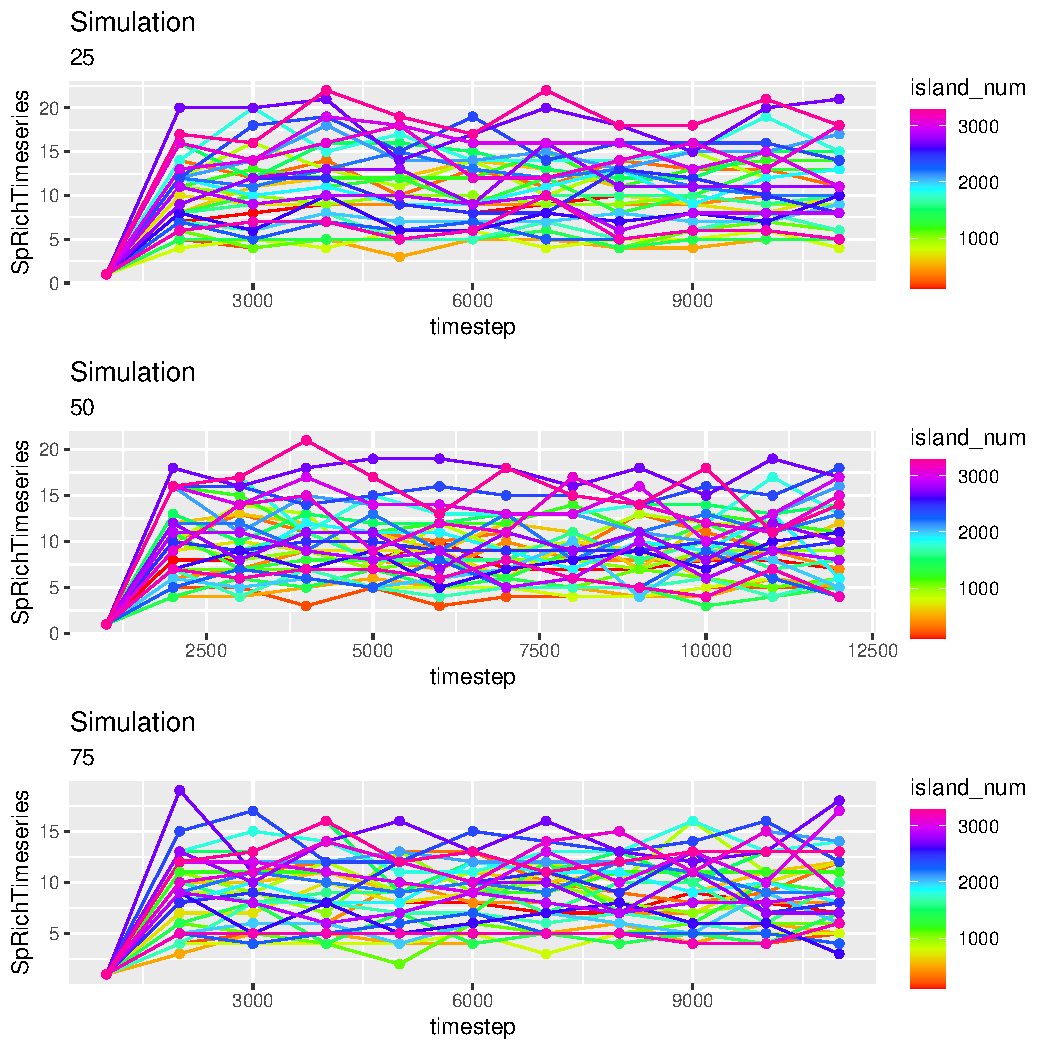
\includegraphics[scale=0.5]{../../Results/Simulation/TimeseriesPlot.pdf}
  \caption{Timeseries plot of three simulations}
  \label{fig:Timeseries plot}
\end{figure}

I used data from 3375 different combinations of parameters (15 migration rates, 15 number of niches, 15 size niches), repeated for 100 simulations, with a total of 337 500 simulated islands. 

\subsection{Within Simulation Results}

\subsubsection{Repeatability}
The sum of squared variance among simulations was 5 129 826 (among\_SS). The sum of squared variance within simulations were 10 481 (within\_SS). The repeatability of the simulation was calculated as among\_SS/(within\_SS + among\_SS) = 97.9 or 98\%. 

\subsubsection{Collinearity}

\begin{figure}[h!]
  \centering
  \begin{subfigure}[b]{0.4\linewidth}
    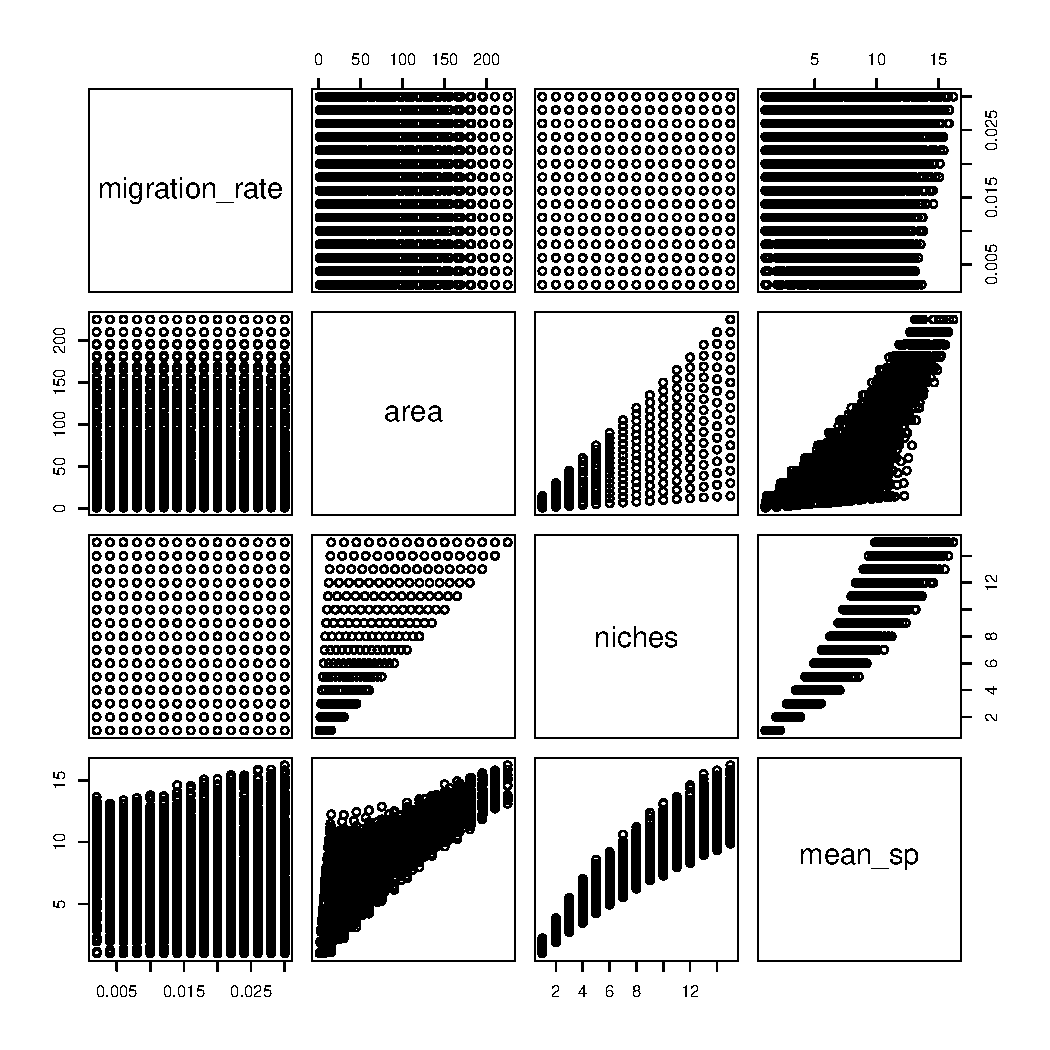
\includegraphics[width=\linewidth]{../../Results/Simulation/CollinearityPlot_1.pdf}
    \caption{maxArea = 225 units}
  \end{subfigure}
  \begin{subfigure}[b]{0.4\linewidth}
    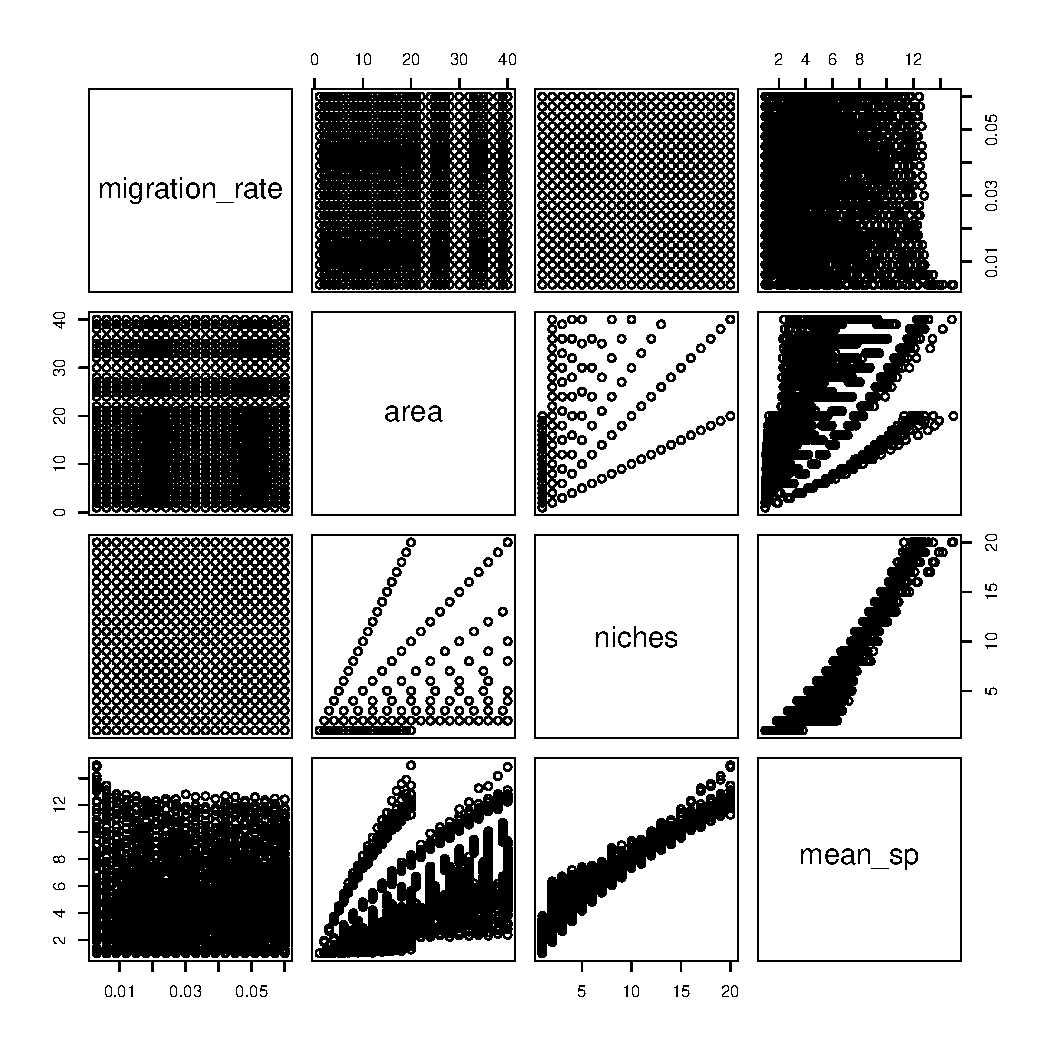
\includegraphics[width=\linewidth]{../../Results/Simulation/CollinearityPlot_10.pdf}
    \caption{maxArea = 22 units}
  \end{subfigure}
  \caption{Collinearity plots for full data set (a) and reduced data set (b)}
  \label{fig:Collinearity}
\end{figure}

The collinearity statistic for migration rate and area was 0, migration rate and niches 0. Migration rate and species richness 0.104. Collinearity scores for area and niches for the whole dataset was 0.661. The independent variables were all positively correlated, with number of niches being a better predictor of species richness than area or migration rate. The VIF score for collinearity between niches and area was 1.77. The standard errors of number of niches are therefore inflated by 1.33, which is within an acceptable range. 

\subsubsection{Linear Regression Analysis}

\begin{figure}[h!]
\centering
  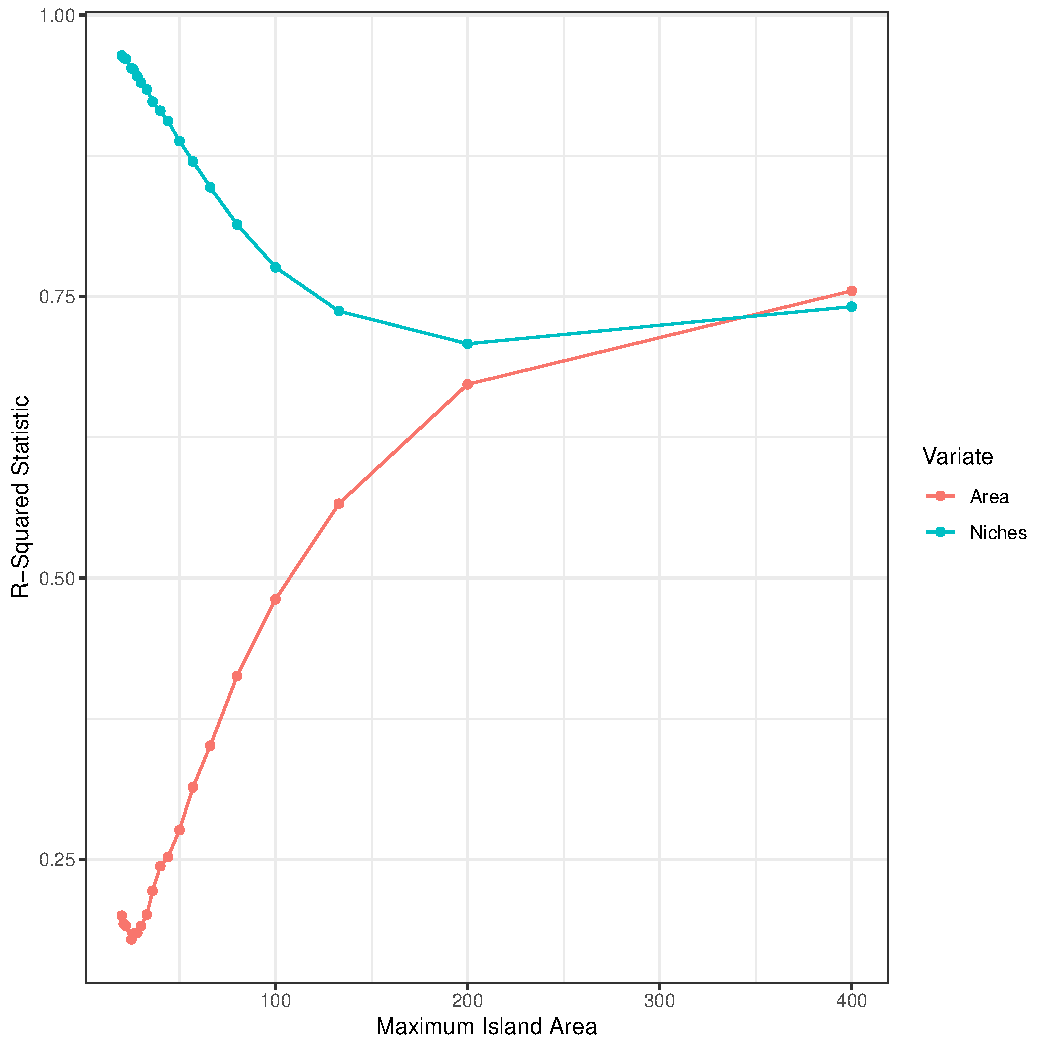
\includegraphics[scale=0.5]{../../Results/Simulation/LMRSquared.pdf}
  \caption{Change of R-squared statistic for number of niches and island area, with changing island size}
  \label{fig:R-Squared statistic}
\end{figure}

The linear model results of species richness and z-transformed area gave an r-squared value of 0.679 with a p-value $<$ 0.001. This indicated that area was a positive, statistically significant relationship between area and species richness. \bigskip

Visual inspection of residual vs fitted results for the entire dataset (max area 225) indicates that lower fitted values had a greater residual range than higher fitted values. The normal Q-Q plot showing standardised residuals plotted against the quantiles they are supposed to lie in fall along a relatively straight line.  \bigskip

The r-squared value for the area/species richness linear model reduced from 0.679 to 0.15 as maximum island area was reduce from 225 units to 22 units. This indicated that area had a weaker positive relationship with species richness as island area decreased. \bigskip

\begin{figure}[h!]
  \centering
  \begin{subfigure}[b]{0.4\linewidth}
    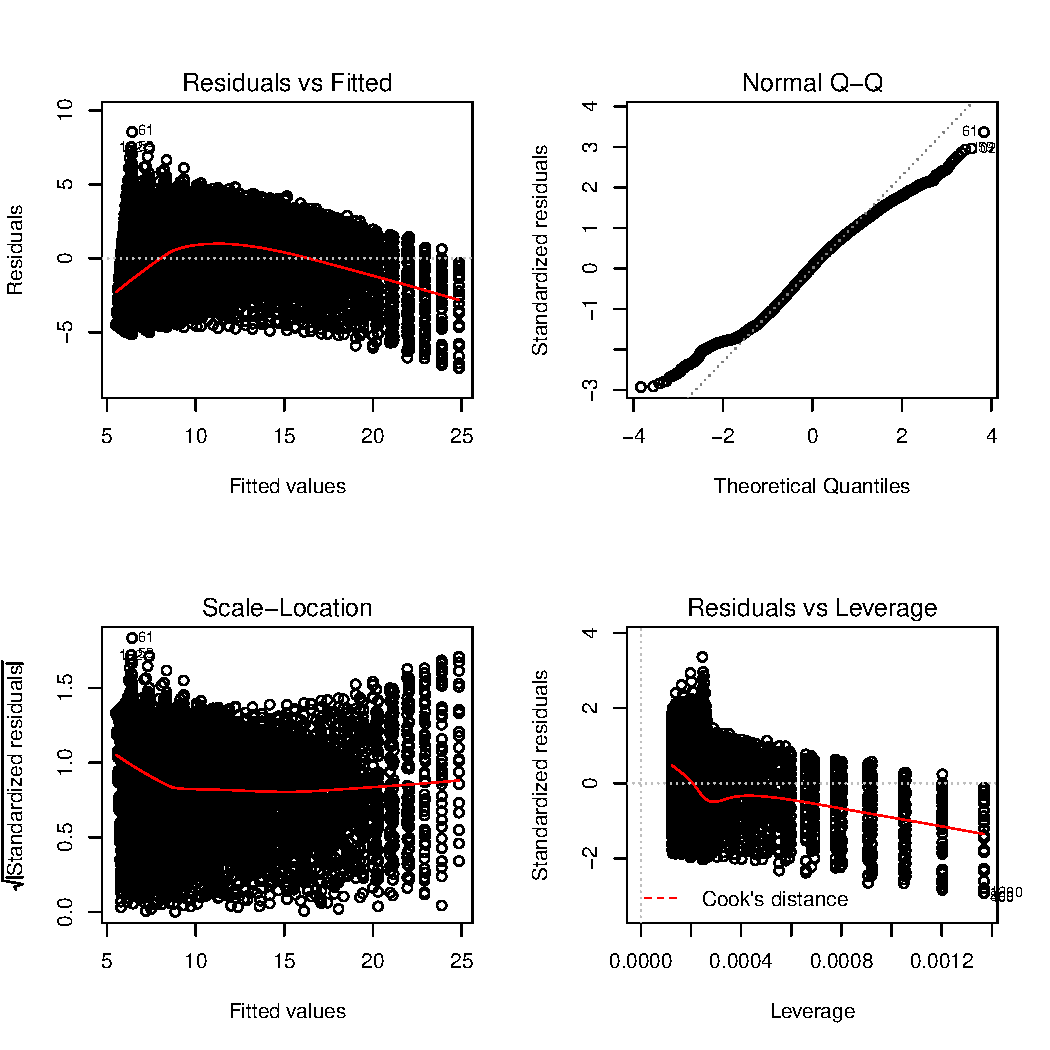
\includegraphics[width=\linewidth]{../../Results/Simulation/AreaSpeciesLmPlot_1.pdf}
    \caption{maxArea = 225 units}
  \end{subfigure}
  \begin{subfigure}[b]{0.4\linewidth}
    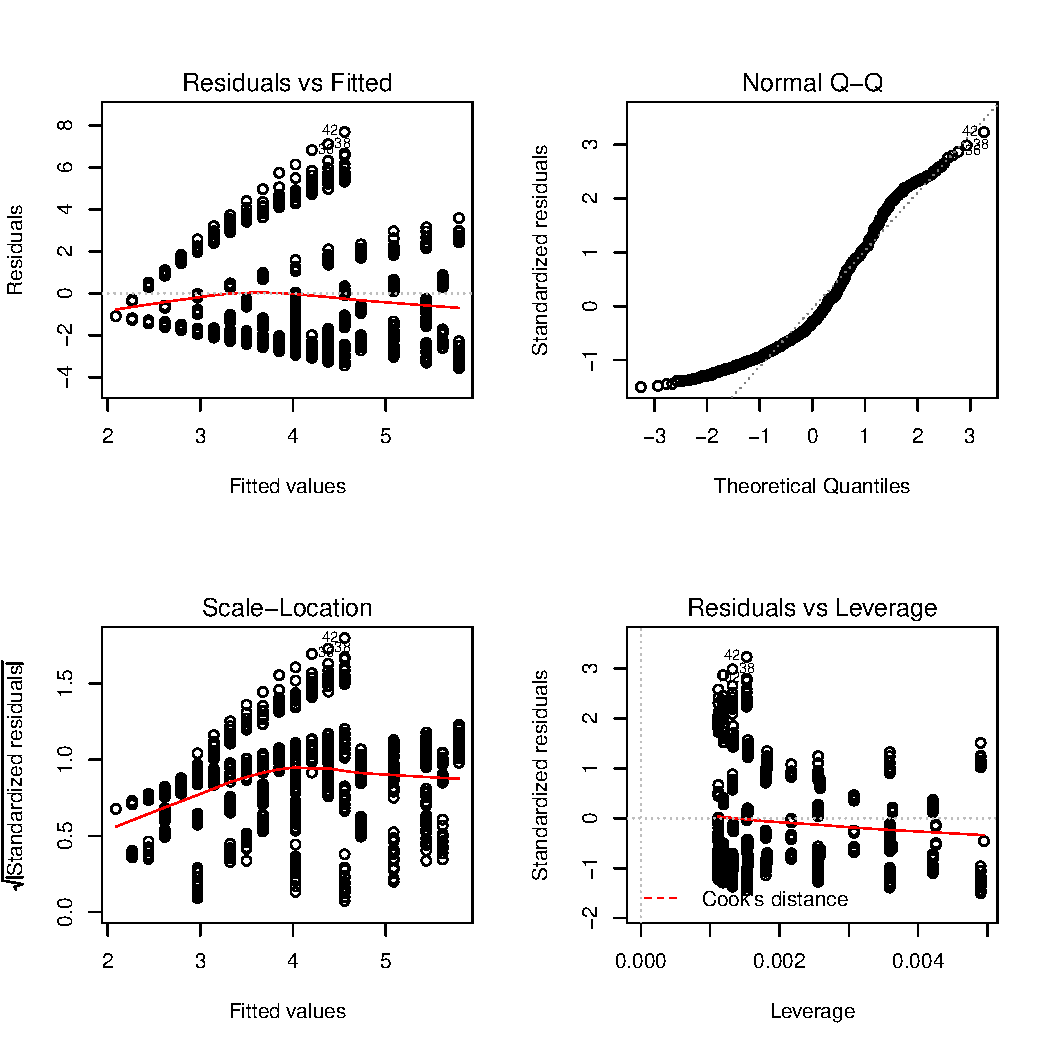
\includegraphics[width=\linewidth]{../../Results/Simulation/AreaSpeciesLmPlot_10.pdf}
    \caption{maxArea = 22 units}
  \end{subfigure}
  \caption{Model validation: Residuals plots of area and species richness linear models with full data set and reduced data set}
  \label{fig:Model validation area/species LM}
\end{figure}

Visual inspection of the residual vs fitted plot for the most reduced dataset (max area 22 units) indicated that higher fitted values had a greater residual range than lower fitted values. The normal Q-Q plot followed a relatively straight line. \bigskip

The linear model result of species richness and z-transformed niches gave an r-squared value of 0.89 with a p-value $<$ 0.001. This indicated that niches have a positive, statistically significant relationship with species richness. \bigskip

\begin{figure}[h!]
  \centering
  \begin{subfigure}[b]{0.4\linewidth}
    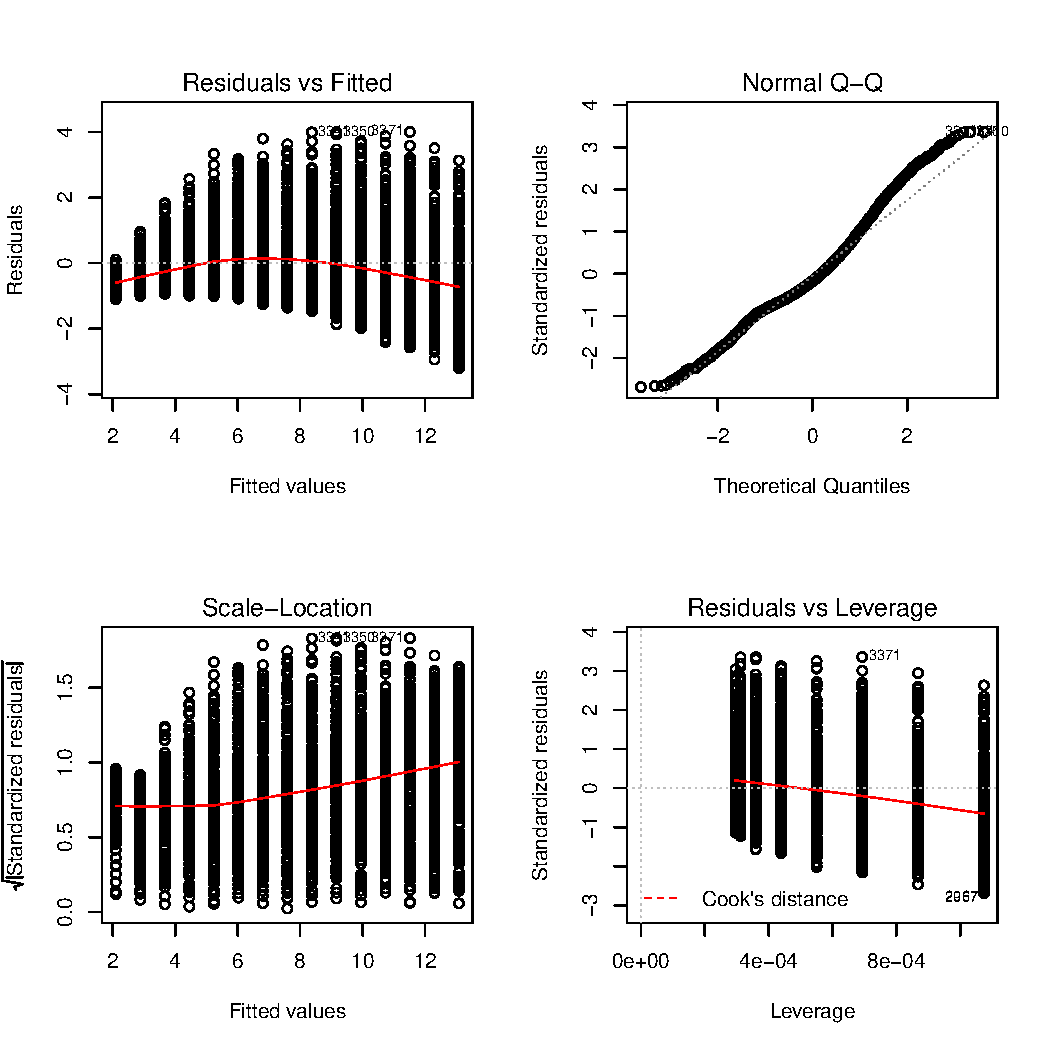
\includegraphics[width=\linewidth]{../../Results/Simulation/NicheSpeciesLmPlot_1.pdf}
    \caption{maxArea = 225 units}
  \end{subfigure}
  \begin{subfigure}[b]{0.4\linewidth}
    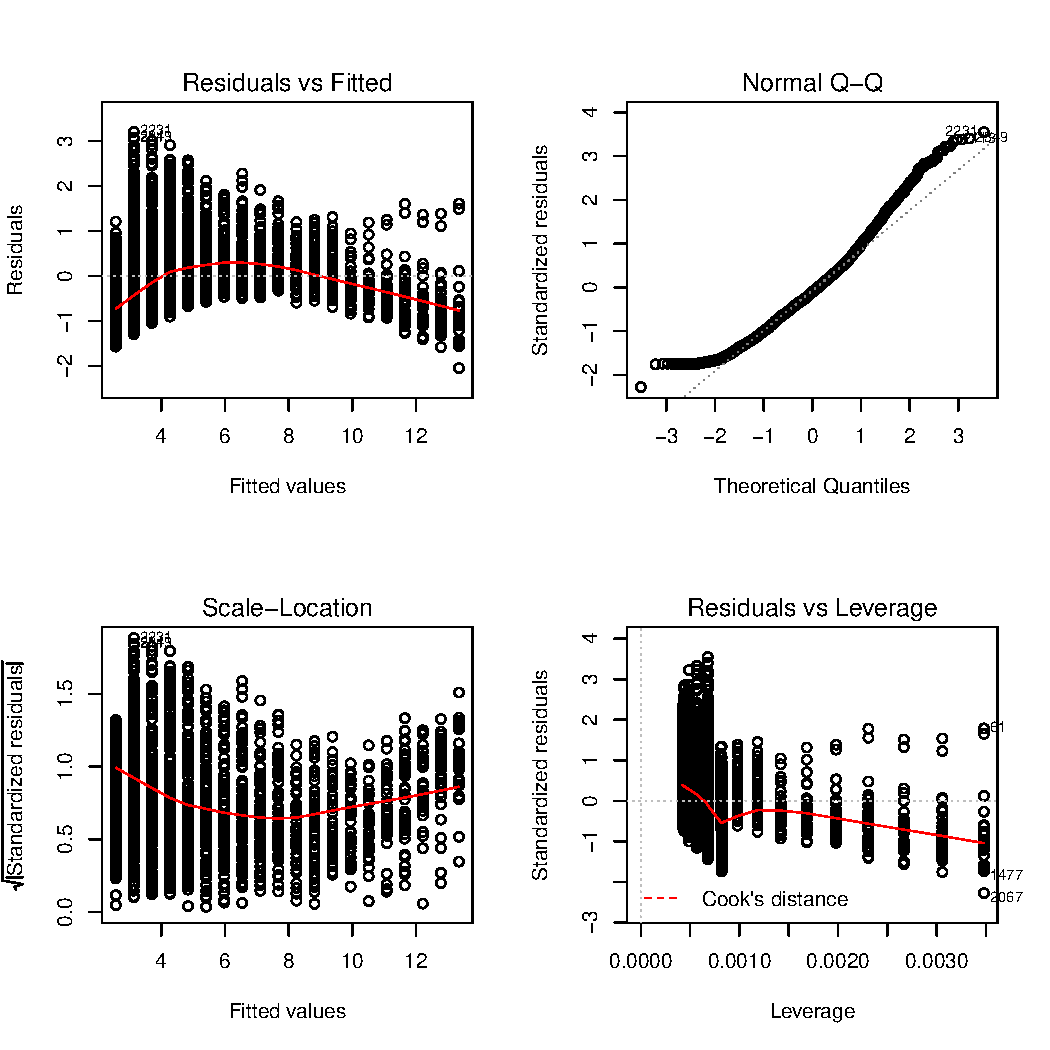
\includegraphics[width=\linewidth]{../../Results/Simulation/NicheSpeciesLmPlot_10.pdf}
    \caption{maxArea = 22 units}
  \end{subfigure}
  \caption{Model validation: Residuals plots of niche and species richness linear models with full data set and reduced data set}
  \label{fig:Model validation niche/species LM}
\end{figure}

Visual inspection of the residual vs fitted plot for the entire dataset indicated that higher fitted values had a greater residual range than lower fitted values. The normal Q-Q plot followed a relatively straight line. \bigskip

The r-squared value for niches/species richness linear model increased from 0.89 to 0.977 as maximum island area was reduced from 225 units to 22 units. This indicated that number of niches had a stronger positive relationship with species richness as island area decreased. \bigskip

Visual inspection of the residual vs fitted plot for the most reduced dataset showed fairly randomly distributed data points. The normal Q-Q plot followed a relatively straight line.  \bigskip

\subsubsection{Multivariate Regression Analysis}
Multivariate analysis results for the whole dataset showed that the combined effects of number of niches, island area and migration rate gave an r-squared value of 0.972. The combined effects of niche and area gave an r-squared value of 0.961. This indicates that migration rate had a weak positive effect on species richness across the entire dataset.  \bigskip

\begin{figure}[h!]
  \centering
  \begin{subfigure}[b]{0.4\linewidth}
    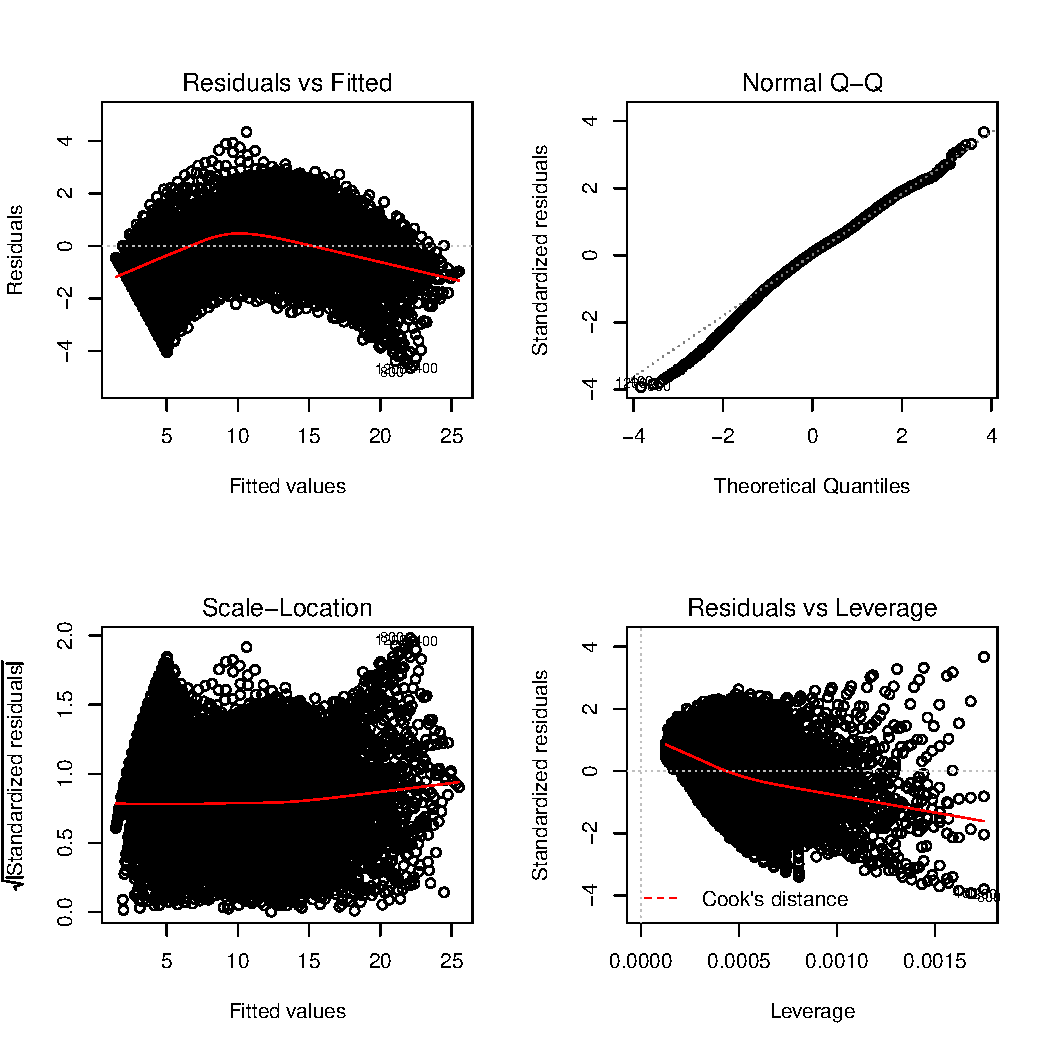
\includegraphics[width=\linewidth]{../../Results/Simulation/NicheAreaMigrationLmPlot_1.pdf}
    \caption{maxArea = 225 units}
  \end{subfigure}
  \begin{subfigure}[b]{0.4\linewidth}
    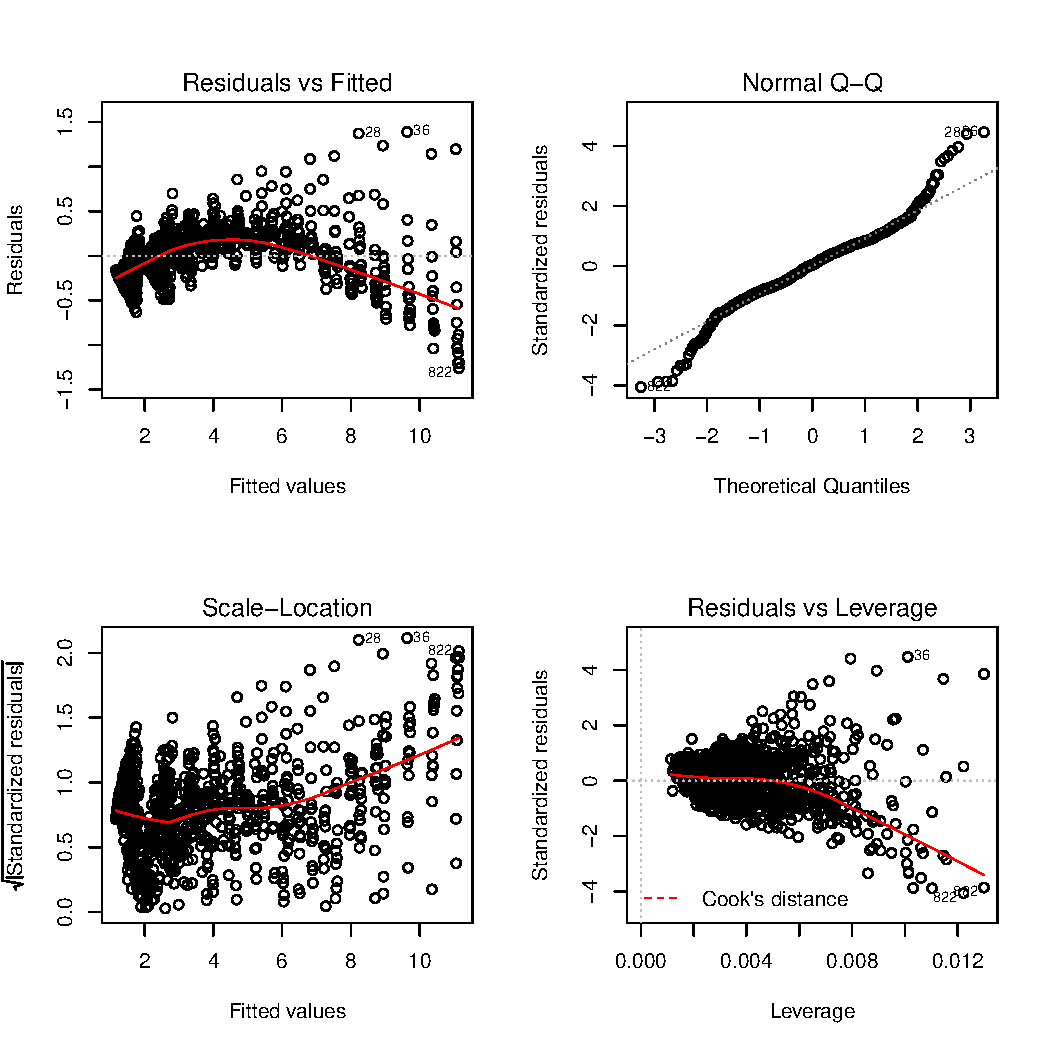
\includegraphics[width=\linewidth]{../../Results/Simulation/NicheAreaMigrationLmPlot_10.pdf}
    \caption{maxArea = 22 units}
  \end{subfigure}
  \caption{Model validation: Residuals plots of multivariate analysis of niche, area, migration and species richness with full data set (a) and reduced data set (b)}
  \label{fig:Model validation multivariate 1}
\end{figure}

\begin{figure}[h!]
  \centering
  \begin{subfigure}[b]{0.4\linewidth}
    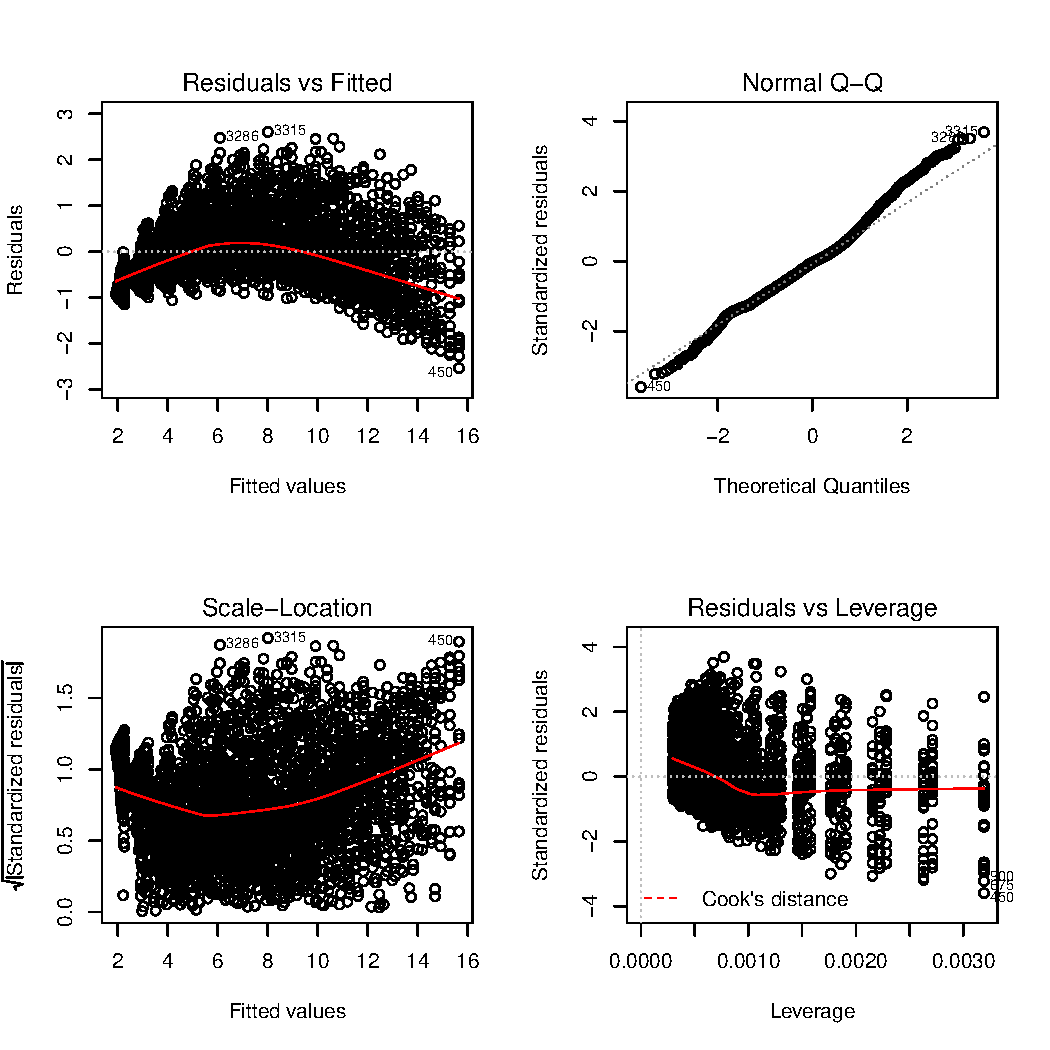
\includegraphics[width=\linewidth]{../../Results/Simulation/NicheAreaLmPlot_1.pdf}
    \caption{maxArea = 225 units}
  \end{subfigure}
  \begin{subfigure}[b]{0.4\linewidth}
    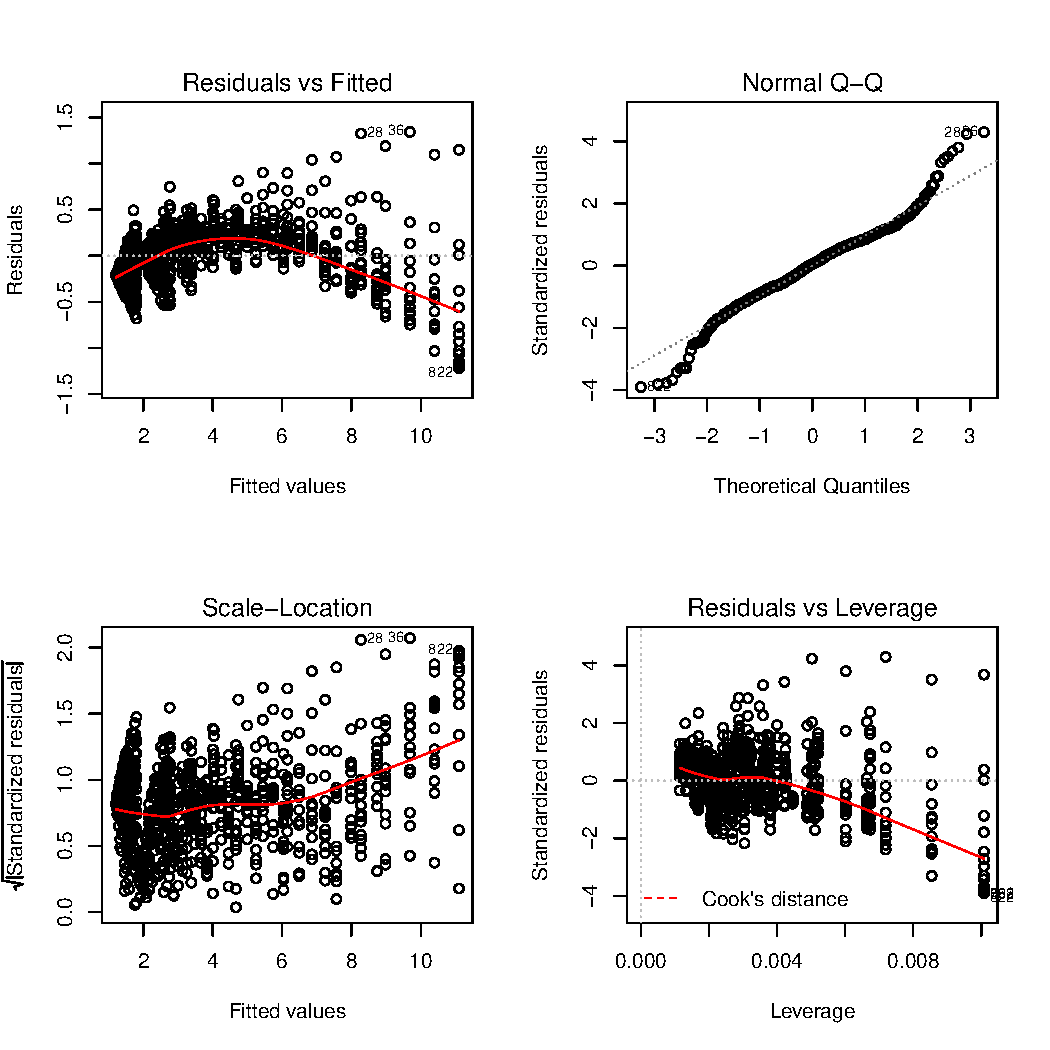
\includegraphics[width=\linewidth]{../../Results/Simulation/NicheAreaLmPlot_10.pdf}
    \caption{maxArea = 22 units}
  \end{subfigure}
  \caption{Model validation: Residuals plots of multivariate analysis of niche, area and species richness with full data set (a) and reduced data set (b)}
  \label{fig:Model validation multivariate 2}
\end{figure}


Visual inspection of the residual results for the linear model showed that the residuals (distances between species richness and calculated regression line) are somewhat randomly distributed. The Q-Q plot showing standardised residuals plotted against the quantiles they are supposed to lie within, gives a relatively straight line. \bigskip

Multivariate analysis results for the most reduced dataset showed that the combined effects of number of niches, island area and migration rate, gave an r-squared value of 0.985. The combined effects of niche and area gave an r-squared value of 0.985, indicating that migration rate had no effect on species richness at smaller island sizes. \bigskip

Distribution of the residuals 

\subsection{Simulation/Model Results}

\subsubsection{Outliers}

\begin{figure}[h!]
  \centering
  \begin{subfigure}[b]{0.4\linewidth}
    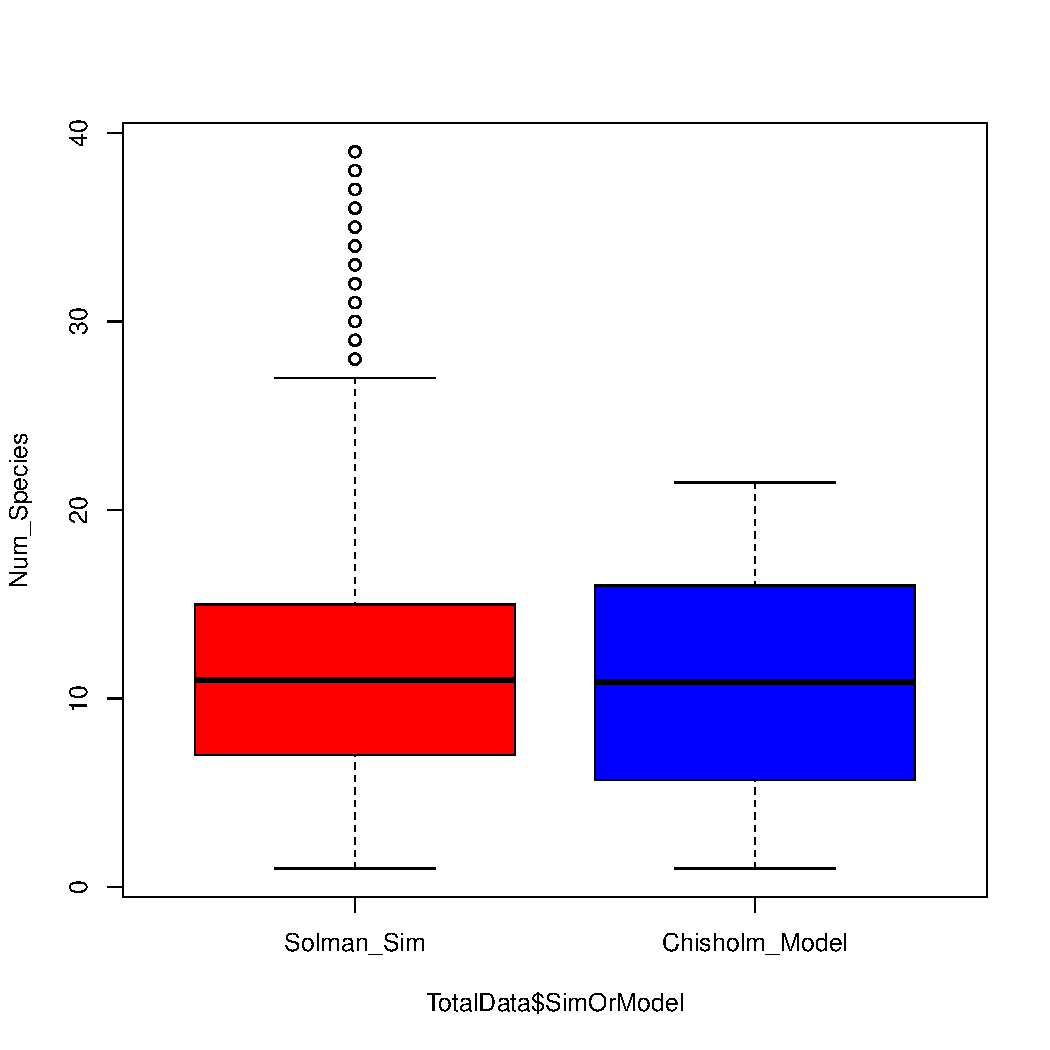
\includegraphics[width=\linewidth]{../../Results/Simulation/SolmanChisholmBoxplot_1.pdf}
    \caption{maxArea = 225 units}
  \end{subfigure}
  \begin{subfigure}[b]{0.4\linewidth}
    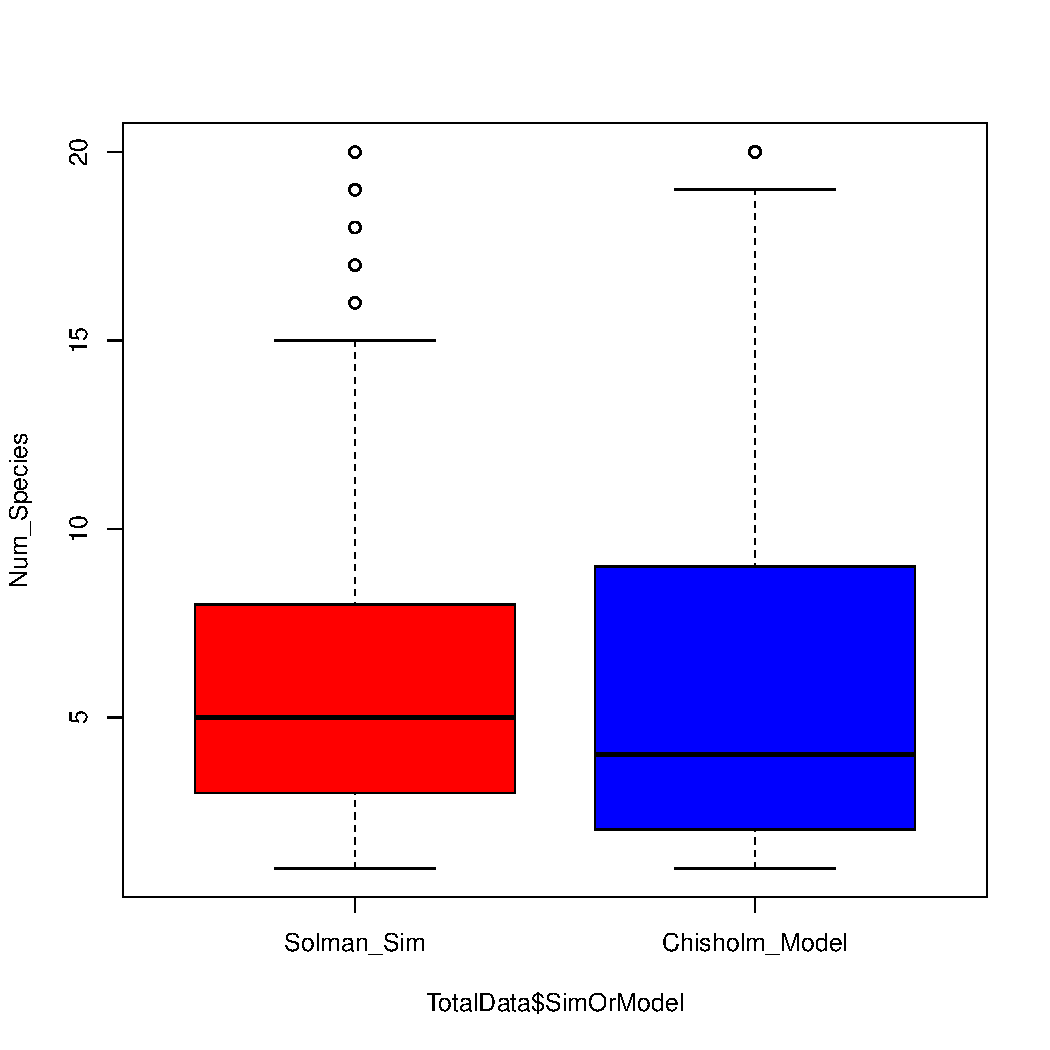
\includegraphics[width=\linewidth]{../../Results/Simulation/SolmanChisholmBoxplot_10.pdf}
    \caption{maxArea = 22 units}
  \end{subfigure}
  \caption{Boxplot of simulation and model estimation data for the full data set and area reduced data set}
  \label{fig:boxplots}
\end{figure}

When comparing boxplots of simulated and estimated species richnesses, the simulation boxplot appeared to show outlying data points. On examining the data, the plotted points represented 569 islands that had species richness values greater than 20. As the number of islands present in this outlier group was so high, it was inappropriate to remove them from the data set as they represent a significant contrinution to the overall mean. Moreover, there was not a sudden jump in values from those within the quartile ranges of the boxplot to those indicated as outliers. It is for this reason the boxplot appears to be misleading.  

\subsubsection{Mean, range, variance, standard deviation and standard error}

\begin{figure}
\centering
  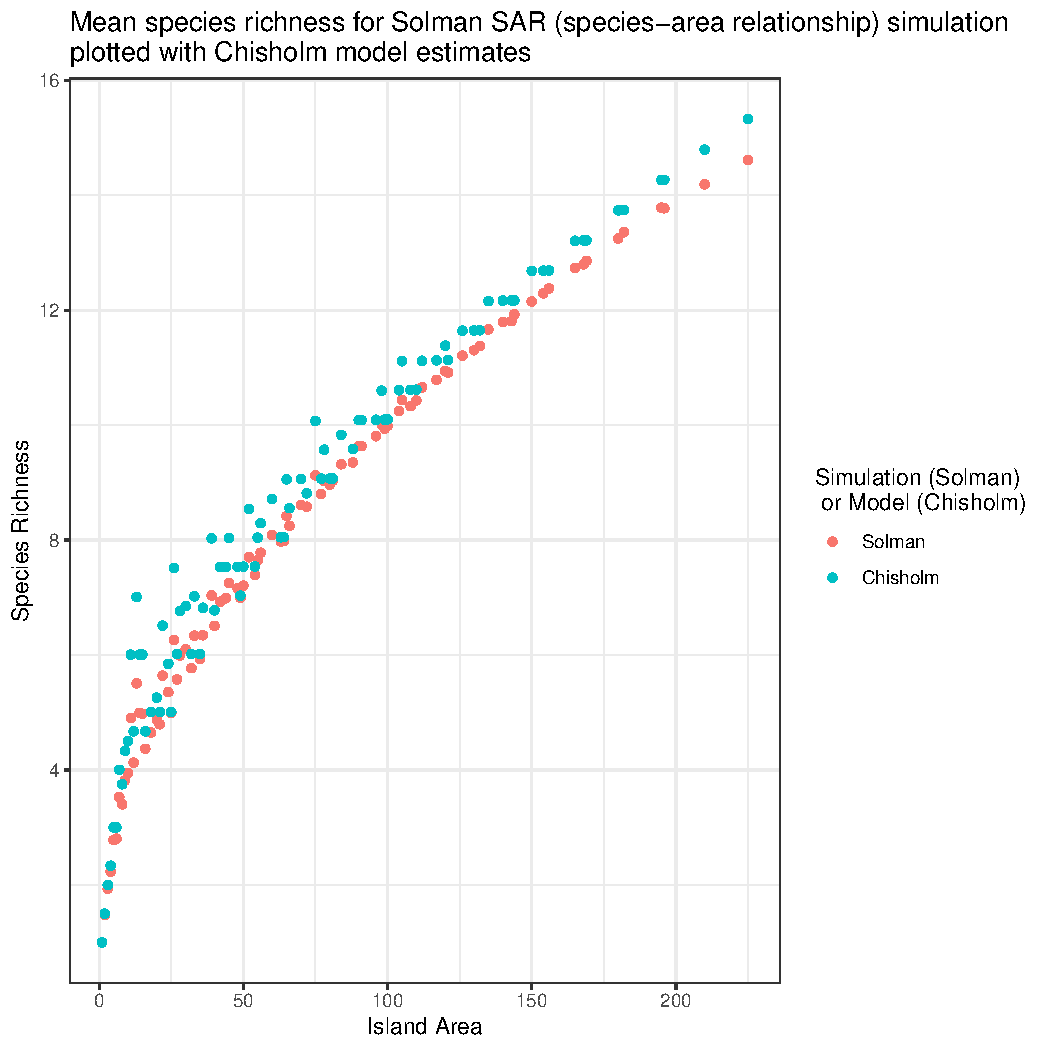
\includegraphics[scale=0.5]{../../Results/Simulation/MeanResultsPlot.pdf}
  \caption{Mean simulation data with model data}
  \label{fig:MeanPlot}
\end{figure}

The mean number of species on a simulated island was (SD, SE, range)
The mean number of species estimated by the model directly was (SD, SE, range)

\subsubsection{Paired-sample t-Test}
The paired-sample t-test results for the full dataset was
The paired sample t-test results for the decreasing dataset was

\subsubsection{Non-Linear Least Squares Fitting}

\begin{figure}
\centering
  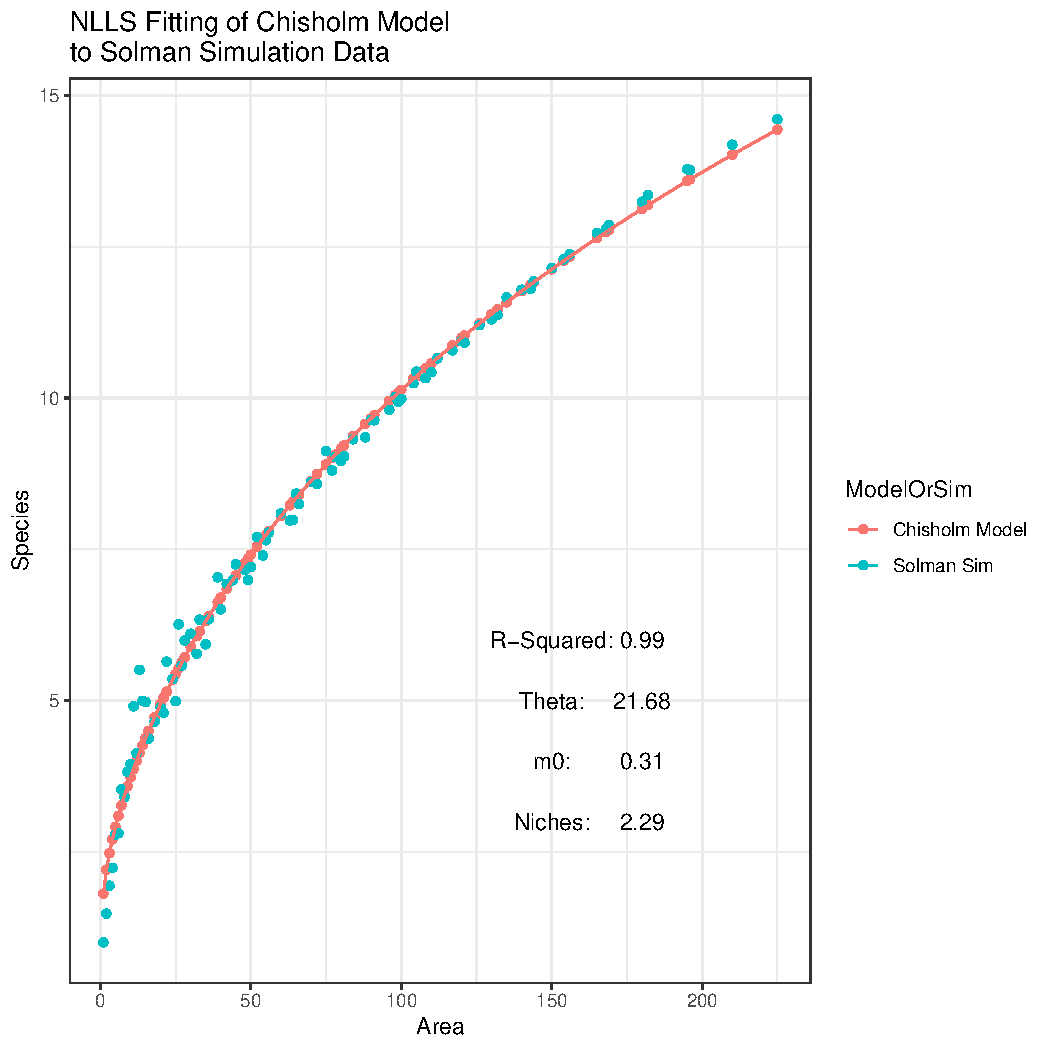
\includegraphics[scale=0.5]{../../Results/Simulation/NLLSFit.pdf}
  \caption{Simulation data with NLLS fitted model data}
  \label{fig:NLLS}
\end{figure}

The mean number of species estimated by the model using NLLS fitting was (SD, SE, range)
The R-squared value of the fitting was 
The p-value from the fitting was 


\end{document}